\section{Visualization}

In order to create a visualization of the algorithms described in the previous sections, a 3D model of the floor plan of the museum was created. First, this floor plan is converted into an SVG image so it can easily be altered in Python. Working this way makes it possible to dynamically create an HTML page showing the SVG floor plan and the currently analyzed frame along with the detected paintings. Because some operations need a lot of processing power, two separate processes are spawned. One process handles the painting detection, the other one handles the room prediction and the visualization of the HTML page in a webview. One of the major points of attention during the creation of the visualization was performance, hence the HTML file is never written to disk in order to bypass the I/O operations. Therefor the HTML page is always kept in memory. The detection process uses interprocess communication to send the detected paintings and the currently processed frame to the second process. This process then updates the Hidden Markov model as well as the HTML page and shows the result in a webview. An example of this webview is shown in \figureref{fig:webview}. Besides showing the floor plan and the image, other information is shown as well. This includes information about the predicted room, which is also visualized in red on the floor plan, a probability for this prediction, the currently processed video's name and the currently analyzed frame.

\begin{figure}
    \centering
    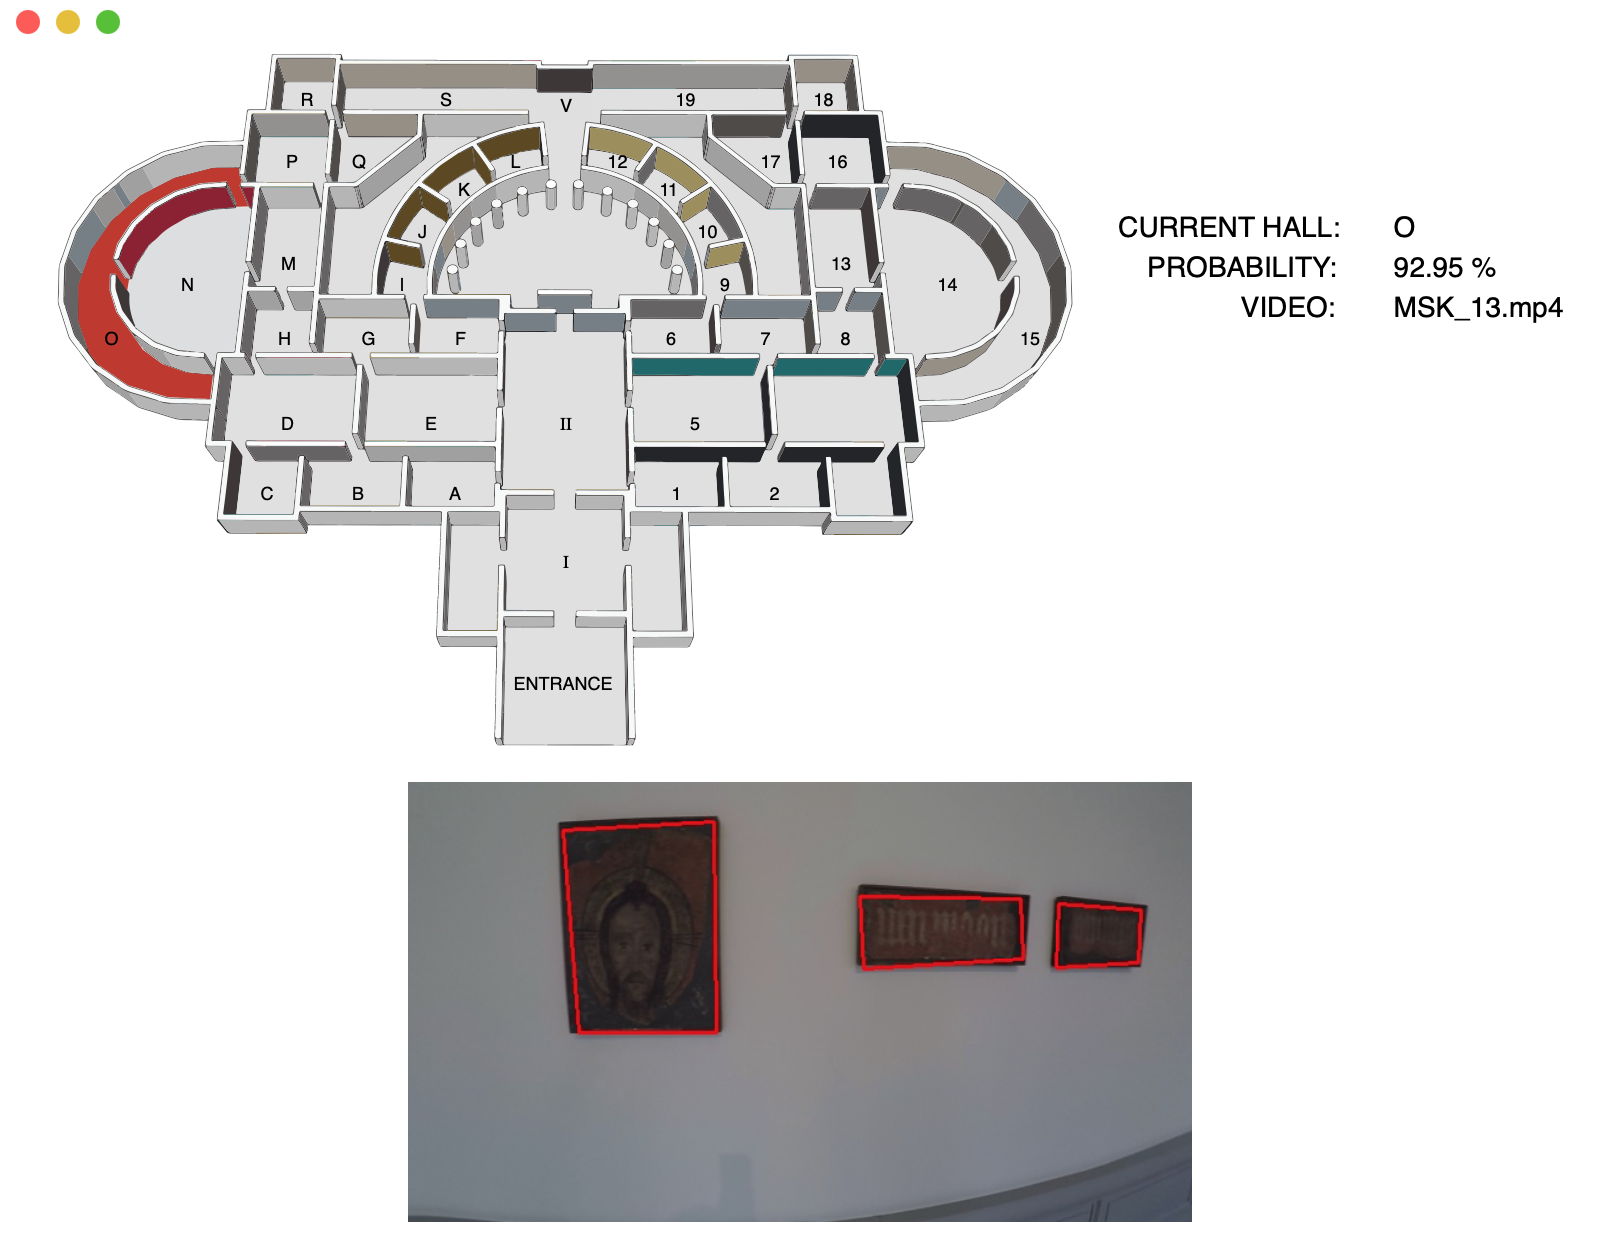
\includegraphics[width=0.6\linewidth]{visualization.png}
    \label{fig:webview}
    \caption{Modern visualization of the floor plan}
\end{figure}

